\documentclass{standalone}

%----------------------------------------------------------------------------------------------%
%                                 Packages and basic declarations
%----------------------------------------------------------------------------------------------%

\usepackage[utf8]{inputenc}
\usepackage{pgfplots}
\usepackage{tikz}


%----------------------------------------------------------------------------------------------%
%----------------------------------------------------------------------------------------------%
%                                            DOCUMENT STARTS
%----------------------------------------------------------------------------------------------%
%----------------------------------------------------------------------------------------------%

\begin{document}


%Tikz picture starts%

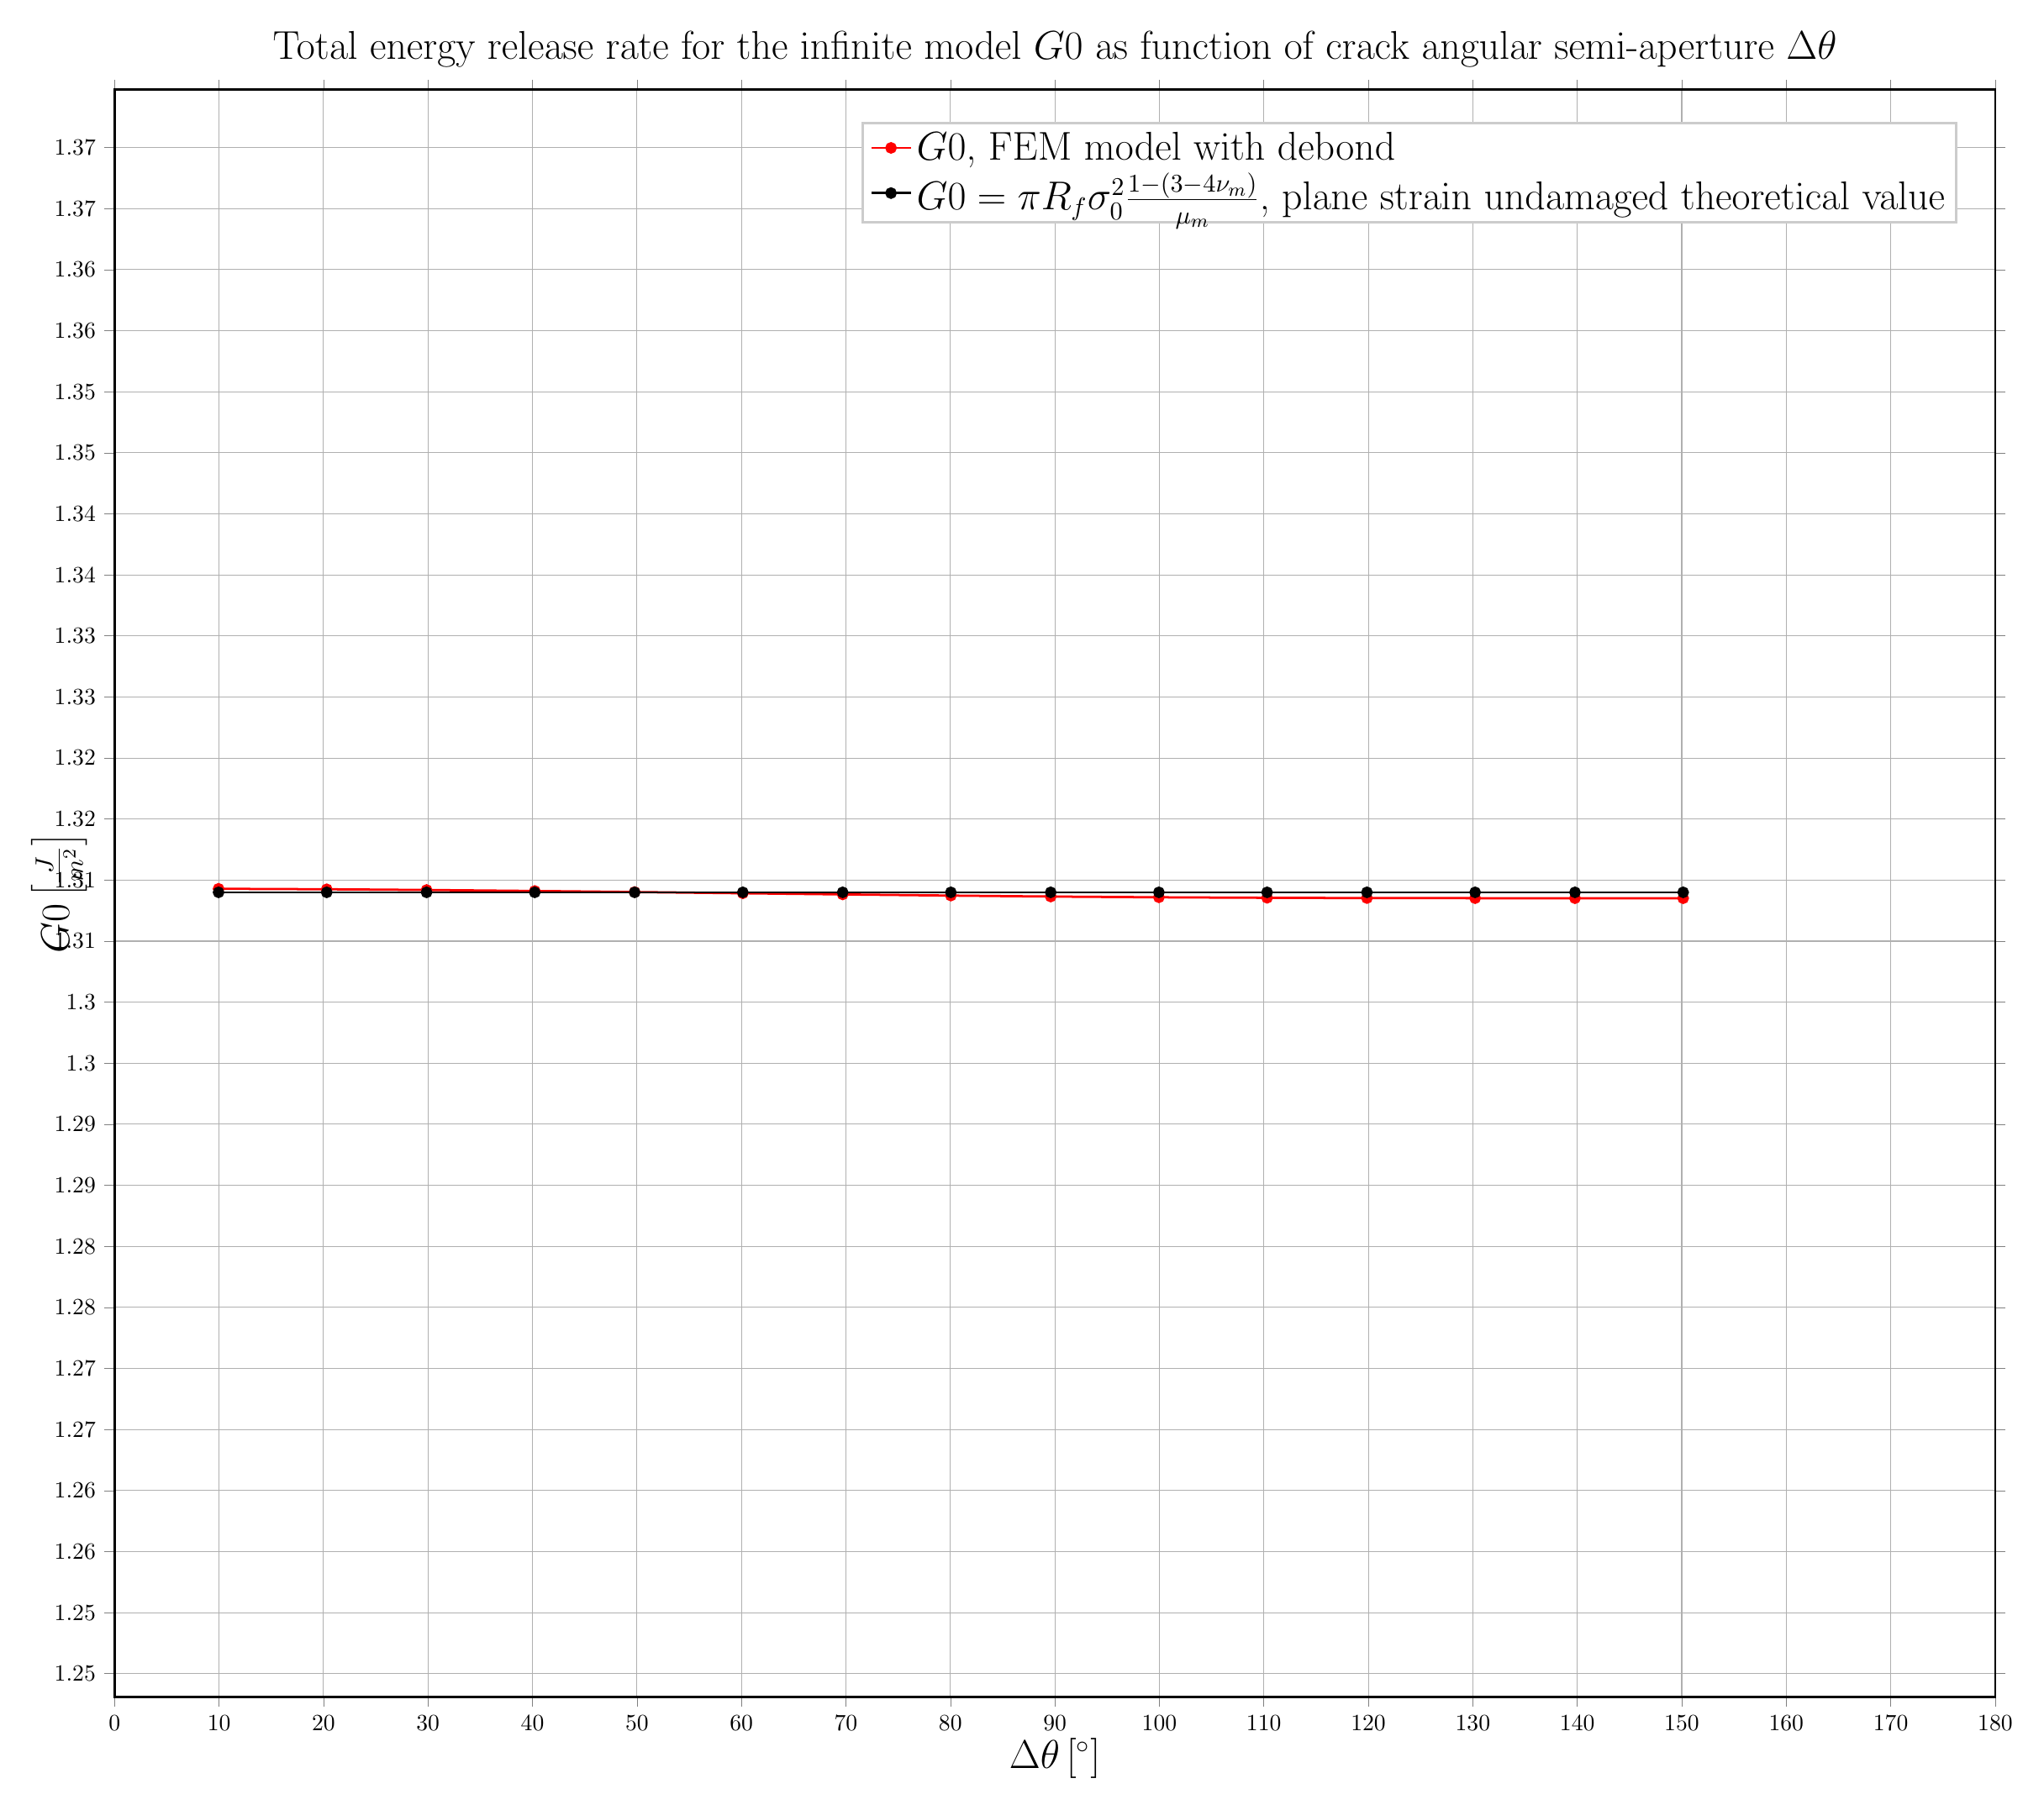
\begin{tikzpicture}

%Tikz axis starts%

\begin{axis}[width=30cm,
title={Total energy release rate for the infinite model $G0$ as function of crack angular semi-aperture  $\Delta\theta$},
title style={font=\fontsize{16}{8}\selectfont},
xlabel style={at={(axis description cs:0.5,-0.02)},anchor=north,font=\fontsize{16}{8}\selectfont},
ylabel style={at={(axis description cs:-0.01,.5)},anchor=south,font=\fontsize{16}{8}\selectfont},
xlabel={$\Delta\theta\left[^{\circ}\right]$},ylabel={$G0\left[\frac{J}{m^{2}}\right]$},
xmin=0.0,
xmax=180.0,
ymin=1.2430890622,
ymax=1.3747504609,
tick align=outside,
tick label style={font=\normalsize},
xtick={0.0,10.0,20.0,30.0,40.0,50.0,60.0,70.0,80.0,90.0,100.0,110.0,120.0,130.0,140.0,150.0,160.0,170.0,180.0},
xmajorgrids,
x grid style={lightgray!92.026143790849673!black},
ymajorgrids,
y grid style={lightgray!92.026143790849673!black},
line width=0.35mm,
legend style={draw=white!80.0!black,font=\fontsize{16}{12}\selectfont},
legend entries={{$G0$, FEM model with debond},{$G0=\pi R_{f}\sigma_{0}^{2}\frac{1-\left(3-4\nu_{m}\right)}{\mu_{m}}$, plane strain undamaged theoretical value}},
legend cell align={left}
]

\addplot[red,smooth,mark=*]
table{
9.95590315404 1.30928615324
20.3094667517 1.3092465045
29.8671878064 1.30918874723
40.2210818145 1.30910782065
49.7789172749 1.30902118929
60.1328146981 1.30892065631
69.6905306301 1.30882728887
80.044093374 1.30873176676
89.6017683249 1.30865267325
99.9559048047 1.30859178266
110.309467549 1.30854975851
119.867183481 1.30852817807
130.221080904 1.30851818146
139.778919779 1.30851576088
150.132817203 1.30851552439
};

\addplot[black,smooth,mark=*]
table{
9.95590315404 1.308996939
20.3094667517 1.308996939
29.8671878064 1.308996939
40.2210818145 1.308996939
49.7789172749 1.308996939
60.1328146981 1.308996939
69.6905306301 1.308996939
80.044093374 1.308996939
89.6017683249 1.308996939
99.9559048047 1.308996939
110.309467549 1.308996939
119.867183481 1.308996939
130.221080904 1.308996939
139.778919779 1.308996939
150.132817203 1.308996939
};

\end{axis}
%Tikz axis ends%


\end{tikzpicture}
%Tikz picture ends%


\end{document}

%----------------------------------------------------------------------------------------------%
%----------------------------------------------------------------------------------------------%
%                                            DOCUMENT ENDS
%----------------------------------------------------------------------------------------------%
%----------------------------------------------------------------------------------------------%

